
\begin{frame}{The problems...  %
    \onslide<5->{%
      \vspace{-0.94cm} 
      \begin{flushright}
        ... the solution \textcolor{white}{--}
      \end{flushright}
    }
  }

  % http://rrcns.readthedocs.org/en/latest/version_control.html
  % http://www.phdcomics.com/comics.php?f=1323

  \large
  \begin{columns}  
  %%%%
    \begin{column}{0.4\textwidth}
      \vspace{0.46cm}
      \begin{itemize}[leftmargin=2pt]
        \itemsep18pt
        \item<1->[] Which version of my code did I use?
        \item<2->[] What parameters?
        \item<3->[] \enquote{Why did I do that?}
        \item<4->[] \enquote{It worked yesterday.}
      \end{itemize}
      \vspace{3cm}
    \end{column}
    %%%% 
    \begin{column}{0.55\textwidth}
      \vspace{-1.35cm}
      \only<1-4>{
        \vspace{0.4cm}

        \begin{figure}
          \centering        
          \includegraphics[width=6.6cm]{%
            phd_filenames.png}
          \vspace{-0.28cm}
          \captionsetup{justification=centering}
          \caption*{%
            \tiny \enquote{Piled Higher and Deeper} by Jorge Cham
            \href{www.phdcomics.com}{www.phdcomics.com}}
        \end{figure}
      }

      \only<6->{
        \vspace{0.01cm}
        \begin{center}
          \textbf{\textit{laboratory notebook}}
        \end{center}
        \vspace{-1.25cm}
        
        \begin{figure}
          \centering        
          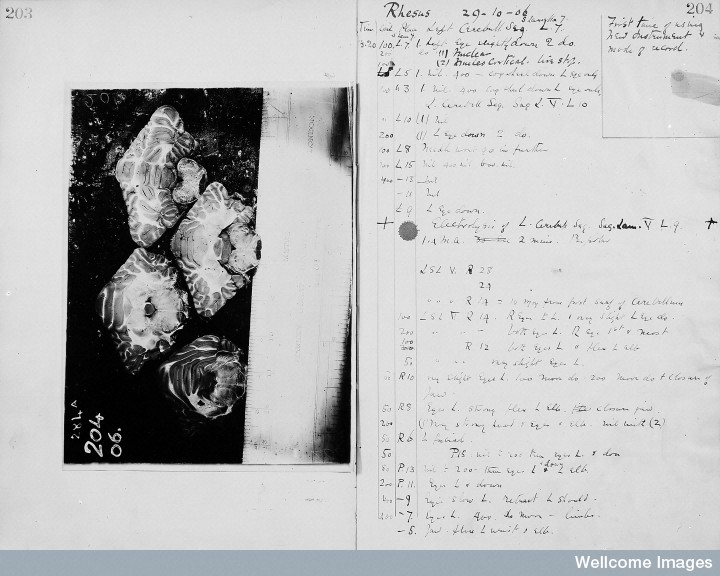
\includegraphics{victor_horsely.jpg}
          % http://wellcomeimages.org/indexplus/image/M0016267.html
          \vspace{-0.28cm}
          \caption*{%
            \tiny \textcopyright Wellcome Library, London 
            \href{http://creativecommons.org/licenses/by/4.0/}{%
              CC BY 4.0}}
        \end{figure}}
      

      \onslide<7->
      \vspace{-0.72cm}
      \begin{center}
        \textit{... in traditional, experiment-based research}.
      \end{center}
    \end{column}
    %%%%
  \end{columns}

\end{frame}


%%% Local Variables: 
%%% mode: latex
%%% TeX-master: "../OpenCon_present"
%%% End: 
